Рендеринг компьютерной графики включает несколько этапов: 
\begin{enumerate}
    \item Моделирование. Создание 3D"=модели объекта или сцены. На этом этапе создают геометрию объектов с помощью полигонов, кривых и других элементов. Используют специализированное программное обеспечение.  
    \item Текстурирование. Добавление текстур и материалов к модели. Текстуры накладывают на модели, чтобы добавить цвет, узоры и детали поверхности. Для точного наложения текстур 3D"=модель разворачивают на плоскую поверхность "--- это называется UV"=развёрткой.
    \item Освещение. Настройка источников света в сцене.  Освещение определяет, как свет взаимодействует с объектами и материалами. Используют различные типы источников света: точечные, направленные, окружающие. Также рассчитывают тени, которые создают объекты при взаимодействии с источниками света.  
    \item Растеризация или трассировка лучей. Преобразование 3D"=сцены в 2D"=изображение с помощью выбранного метода. В зависимости от выбранного метода, происходит растеризация или трассировка лучей.  
    
    \textbf{Растеризация} "--- это одна из групп методов рендеринга, то есть превращение форм трёхмерной сцены в проекцию на двухмерной сетке пикселей, которая выводится на экран пользователя. 
    
    \textbf{Трассировка лучей} "--- более сложный, но реалистичный подход, который отслеживает путь лучей света от камеры до объектов в сцене, учитывая отражения, преломления и тени.
    \item Постобработка. Финальная обработка изображения для улучшения визуального качества.  На этапе постобработки применяют дополнительные эффекты, такие как размытие, наложение фильтров, коррекция цвета. Также могут добавлять эффекты глубины резкости и смягчения, чтобы повысить визуальное качество изображения.
\end{enumerate}

Рассомтрим основы освещения на примере некоторых моделей.

\textbf{Модель Ламберта} (\autoref{fig:lambert}) моделирует идеальное диффузное освещение. Считается, что свет при попадании на поверхность рассеивается равномерно во все стороны. При расчете такого освещения учитывается только ориентация поверхности (нормаль $N$) и направление на источник света (вектор $L$). Рассеянная составляющая рассчитывается по закону косинусов. Для удобства все векторы, описанные ниже, берутся единичными. В этом случае косинус угла между ними совпадает со скалярным произведением:
\begin{figure}[H]
    \centering
    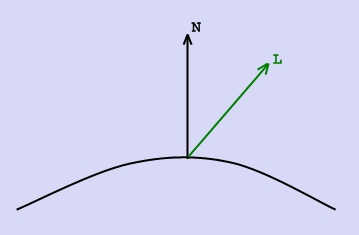
\includegraphics[width=0.59\textwidth]{src/img/lambert.jpg}
    \caption{Модель Ламберта}
    \label{fig:lambert}
\end{figure}

\begin{equation}
    I_{d} = k_{d}\cos(\vec{L}, \vec{N})i_{d} = k_{d}(\vec{L}, \vec{N})i_{d}
\end{equation}
где $I_{d}$ "--- рассеянная составляющая освещенности в точке, $k_{d}$ "--- свойство материала воспринимать рассеянное освещение, $i_{d}$ "--- мощность рассеянного освещения, $\vec{L}$ "--- направление из точки на источник, $\vec{N}$ "--- вектор нормали в точке\cite{light_models}.

Модель Ламберта является одной из самых простых моделей освещения. Она очень часто используется в комбинации других моделей, практически в любой другой модели освещения можно выделить диффузную составляющую. Более"=менее равномерная часть освещения (без присутствия какого"=либо всплеска) как правило будет представляться моделью Ламберта с определенными характеристиками. Данная модель может быть очень удобна для анализа свойств других моделей (за счет того, что ее легко выделить из любой модели и анализировать оставшиеся составляющие).

\textbf{Модель Фонга} (\autoref{fig:fong}) "--- классическая модель освещения. Она представляет собой комбинацию диффузной составляющей (модели Ламберта) и зеркальной составляющей и работает таким образом, что кроме равномерного освещения на материале может еще появляться блик. Местонахождение блика на объекте, освещенном по модели Фонга, определяется из закона равенства углов падения и отражения. Если наблюдатель находится вблизи углов отражения, яркость соответствующей точки повышается.
\begin{figure}[H]
    \centering
    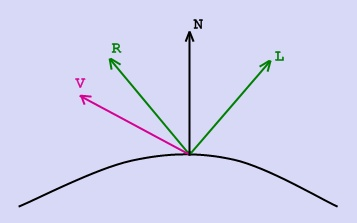
\includegraphics[width=0.59\textwidth]{src/img/fong.jpg}
    \caption{Модель Фонга}
    \label{fig:fong}
\end{figure}

Падающий и отраженный лучи лежат в одной плоскости с нормалью к отражающей поверхности в точке падения, и эта нормаль делит угол между лучами на две равные части. То есть отраженная составляющая освещенности в точке зависит от того, насколько близки направления на наблюдателя и отраженного луча. Это можно выразить следующей формулой:

\begin{equation}
    I_{s} = k_{s}\cos^{\alpha}(\vec{R}, \vec{V})i_{s} = k_{s}(\vec{R}, \vec{V})^{\alpha}i_{s}
\end{equation}
где $I_{s}$ "--- зеркальная составляющая освещенности в точке, $k_{s}$ "--- коэффициент зеркального отражения, $i_{s}$ "--- мощность зеркального освещения, $\vec{R}$ "--- направление отраженного луча, $\vec{V}$ "--- направление на наблюдателя, $\alpha$ "--- коэффициент блеска, свойство материала\cite{light_models}.